\begin{frame}{形状取り込み}
  %
   \begin{columns}[t]
    \begin{column}{0.6\textwidth}
      <今回の形状取り込みの概要>
      \begin{itemize}
        \item[(1)]<1-> PrePoMax を立ち上げ、
		       File→Newでまっさらなモデルを作成
        \item[(2)]<1-> 配布物( ./02-hmsh-shapeから)
		       successful-examples.brepをimport
        \item[(3)]<2-> すべての立体を選択し右クリック
                       「create compound part」で結合
        \item[(4)]<3-> 立体が1つの地続きの形状にまとまる
        \item[(5)]<4-> 元の立体の物性値やメッシュサイズを
		       個別に設定も可能となる
      \end{itemize}
    \end{column}
    \begin{column}{0.4\textwidth}
      \vspace{-7mm}
      \begin{figure}[htbp]
        \begin{center}
          \begin{overlayarea}{7cm}{15cm}
            \only<1>{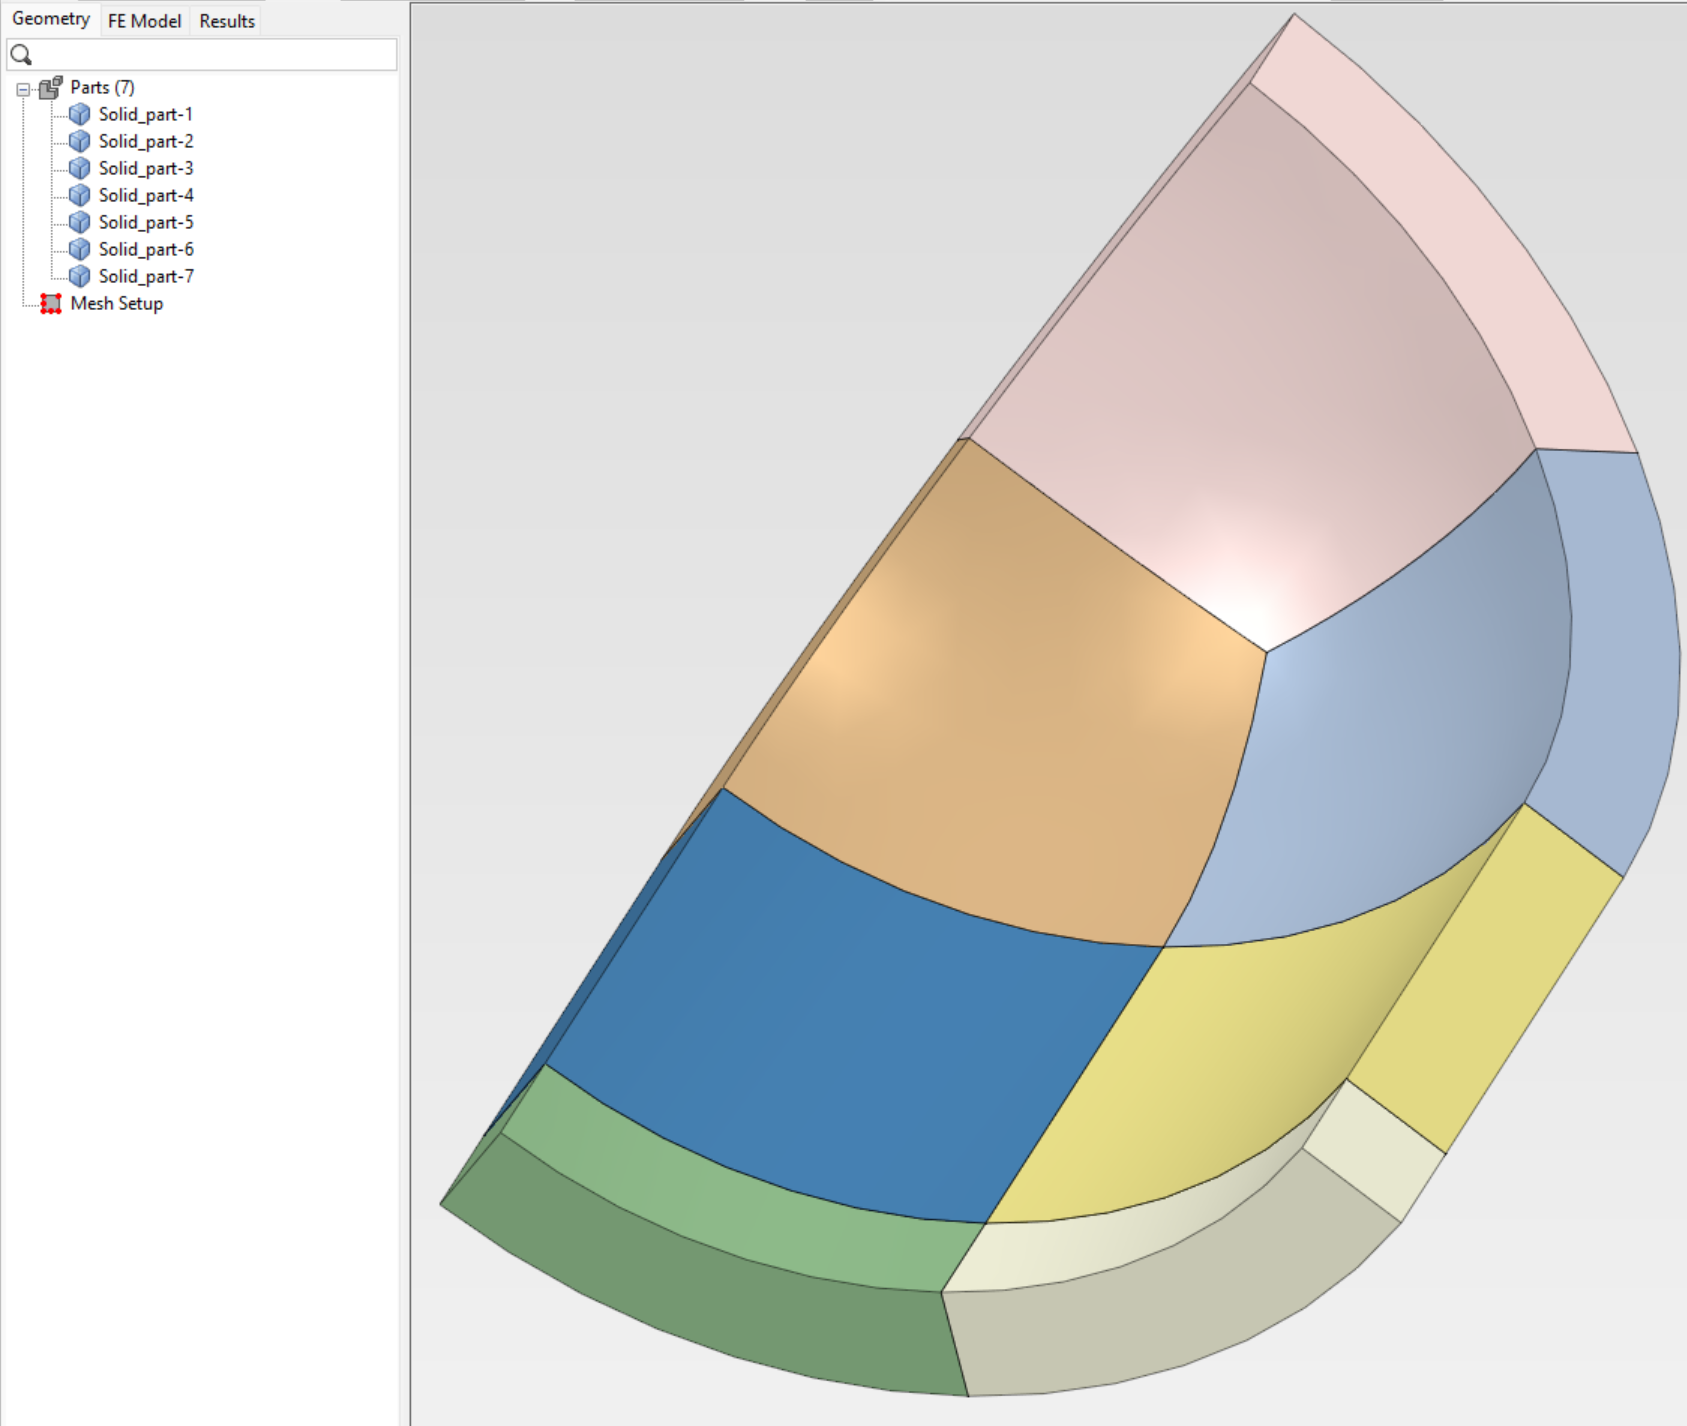
\includegraphics[keepaspectratio,scale=0.30]{images/sc4.png}}
            \only<2>{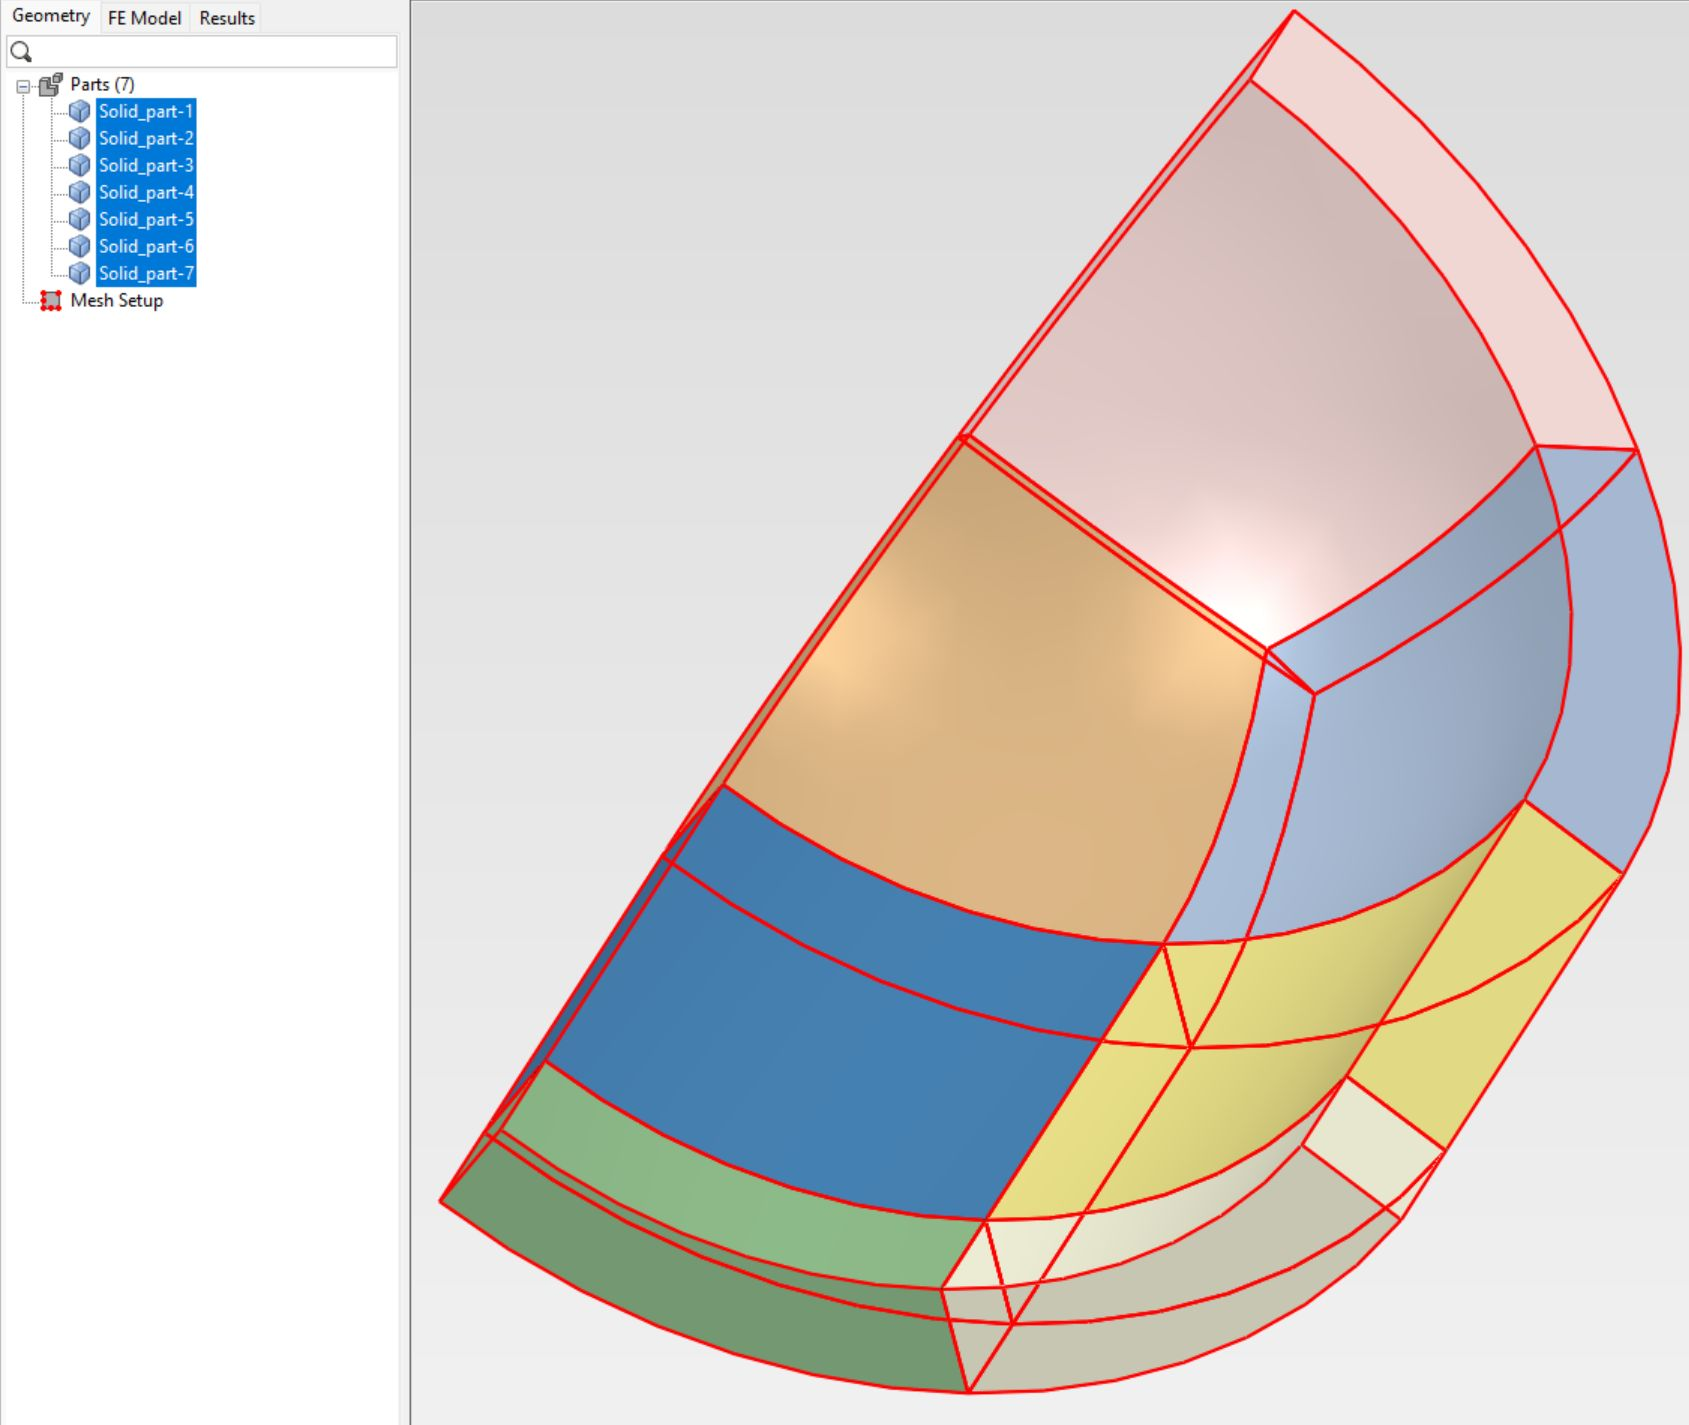
\includegraphics[keepaspectratio,scale=0.30]{images/sc5.png}}
            \only<3->{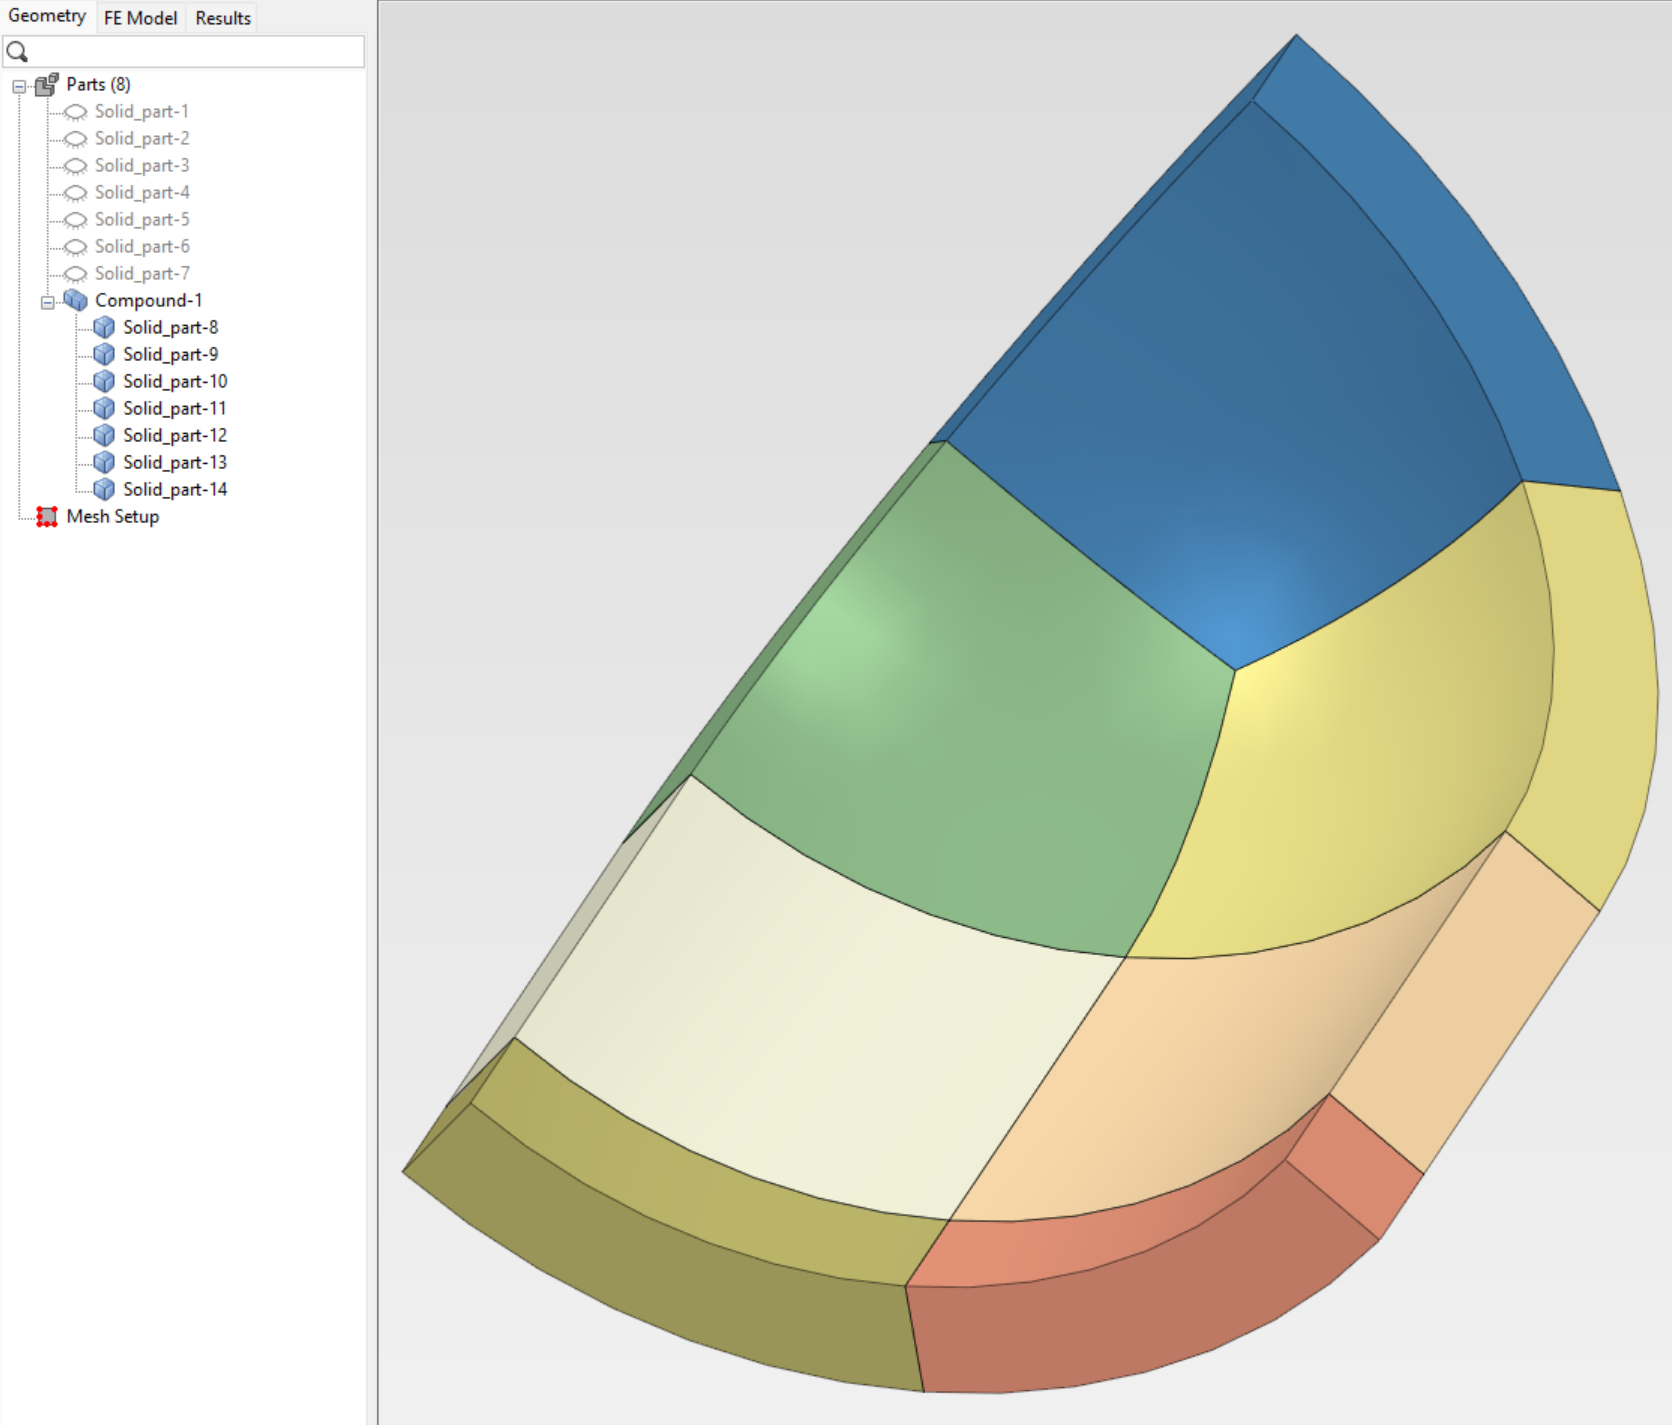
\includegraphics[keepaspectratio,scale=0.30]{images/sc6.png}}
            \caption{形状取り込みの概要}
          \end{overlayarea}
        \end{center}
      \end{figure}
    \end{column}
  \end{columns}
  \only<1>{
    \begin{textblock*}{140pt}(210pt,60pt)
      \begin{tikzpicture}
         \node[rectangle,fill=cud_yellow,text width=70pt,text centered,rounded corners,minimum height=40pt](s) at (1cm,1cm) { \scriptsize 7つの立体が\\取り込まれる};
         \draw[->, draw=cud_red, line width=1pt] (10pt,50pt) -- (30pt,110pt);
      \end{tikzpicture}
    \end{textblock*}
  }
  \only<3>{
    \begin{textblock*}{100pt}(210pt,90pt)
      \begin{tikzpicture}
         \node[rectangle,fill=cud_yellow,text width=70pt,text centered,rounded corners,minimum height=40pt](s) at (1cm,1cm) { \scriptsize ひと塊の\\形状となる};
         \draw[->, draw=cud_red, line width=1pt] (20pt,50pt) -- (40pt,130pt);
      \end{tikzpicture}
    \end{textblock*}
  }
\end{frame}
